\documentclass{./src/gm2}

% \setlength{\titleblockheight}{10cm}%adjust this lenght if it is needed

\usepackage[english]{babel}
\usepackage[utf8]{inputenc}
\usepackage{amsmath,amssymb,amsfonts,bm}
\usepackage{mathrsfs,overpic}
\usepackage[href]{./src/journals}
\usepackage{lscape,xspace}
\usepackage{subfigure}
\usepackage{morefloats}
\usepackage{booktabs}
\usepackage{adjustbox}
\usepackage{graphicx}

%\usepackage{showframe}   

\newcommand{\overbar}[1]{\mkern+2mu\overline{\mkern-2mu#1\mkern-1mu} \mkern+1mu}
\renewcommand{\epsilon}{\varepsilon}
\renewcommand{\rho}{\varrho}
\newcommand{\p}{\ensuremath{\bm{p}}}
\newcommand{\re}{\ensuremath{\Re {\rm e}}}
\newcommand{\im}{\ensuremath{\Im {\rm m}}}
\newcommand{\mean}[1]{\ensuremath{\langle #1 \rangle}}
\newcommand{\bra}[1]{\ensuremath{\langle#1|}}
\newcommand{\ket}[1]{\ensuremath{|#1\rangle}}
\newcommand{\mup}{\mbox{\ensuremath{\mu^+}}}
\newcommand{\mum}{\mbox{\ensuremath{\mu^-}}}
%\newcommand{\MeVc}{\mbox{\ensuremath{\text{MeV}/c}}}
%\newcommand{\GeVc}{\mbox{\ensuremath{\text{GeV}/c}}}
\newcommand{\geant}{{\tt GEANT}}
\newcommand{\wfd}{{\tt WFD}}
\newcommand{\orcad}{{\tt OrCAD}}
\newcommand{\opera}{{\tt OPERA}}
\newcommand{\mars}{{\tt MARS}}
\newcommand{\gbeamline}{{\tt G4Beamline}}
\newcommand{\ea}{{\em et al.}}
\newcommand{\amu}[1][]{\ensuremath{a_{\mu^{#1}}}}
\newcommand{\gm}{\ensuremath{(g-2)}}
\newcommand{\wa}{\mbox{\ensuremath{\omega_a}}}
\renewcommand{\wp}{\mbox{\ensuremath{\omega_p}}}
\newcommand{\wpt}{\mbox{\ensuremath{\widetilde{\omega}_p}}}
\newcommand{\mus}{\mbox{\ensuremath{\mu\text{s}}}}
\newcommand{\Exp}{\mbox{New \g2\ Experiment}}

%% Physics
\newcommand{\xxx}{\textcolor{green}{XXX}\xspace}

\newtheorem{definition}{Definition}
\newtheorem{theorem}{Theorem}

\begin{document}

%opening
\title{Extraction of the muon beam frequency distribution via the Fourier analysis of the fast rotation signal}
\noteid{G-2 Internal}
\version{1.0}
\author[1]{\mail{antoine.chapelain@cornell.edu}{A.~Chapelain}}
\author[1]{\mail{david.rubin@cornell.edu}{D.~Rubin}}
\author[1]{\mail{dms525@cornell.edu}{D.~Seleznev}}

\affil[1]{Cornell University}

\maketitle

\tableofcontents

\section{Introduction}

The Fermilab E989 Muon g-2 experiment aims to measure the anomalous part \amu\ of the magnetic moment of the muon.
The muon acquires a magnetic moment 
\begin{equation} 
\vec{\mu}=g \frac{Q}{2m} \vec{s},
\end{equation} in the presence of an external magnetic field $B$, where $Q$ is the muon electric charge, $\vec{s}$ the muon spin vector 
and $g$  the gyromagnetic ratio. 
The anomalous part of the magnetic moment is defined via the deviation of the gyromagnetic ratio: $g = 2(1+a_\mu)$.

The Muon g-2 experiment relies on the storage of muons inside a weak focusing ring. 
A continuous C-shape dipole magnet occupies the entirety of the storage ring (44.7 m circumference). 
It provides the 1.45 T inward radial focusing to store the muons in the ring. 
The field intensity corresponds to storing muons with the so-called magic momentum of \mbox{3.09 GeV/c} onto the magic orbit (7.112 m radius).
The muons undergo a cyclotron motion in the ring with a revolution frequency of 149.1 ns.

The weak focusing ring does not provide vertical focusing which is essential to store the muons. 
The vertical focusing is provided by four electrostatic quadrupoles (ESQ) located around the ring.
In their rest frame, the muons see the electric field generated by the ESQs as a magnetic field.

The measurement of \amu~ is performed via the measurement of the intensity of the magnetic field in terms of the Larmor precession frequency of a free proton 
\begin{equation}
\hbar \omega_{p} = 2 \mu_{p} | \overrightarrow{B}|,
\end{equation}
and the intrinsic spin precession frequency of the muon \wa. 
The intrinsic muon spin precession frequency is obtained by subtracting the cyclotron frequency $\omega_C$ to the total spin precession frequency of the muon $\omega_S$:
\begin{equation}
\wa = \omega_S - \omega_C.
\end{equation}

Equation~(\ref{eq:amu}) shows the most general vectorial relation between \amu~ and \wa, $B$:
\begin{equation}
\label{eq:amu}
\vec \omega_{a}=\vec \omega_S -\vec\omega_C 
=  - \frac{Qe}{ m}
\left[ a_{\mu} \vec B -  a_{\mu}\left( {\gamma \over \gamma + 1}\right)
(\vec \beta \cdot \vec B)\vec \beta 
- \left( a_{\mu}- {1 \over \gamma^2 - 1} \right) 
{ {\vec \beta \times \vec E }\over c }\right]
\end{equation}

The term proportional to ${\vec \beta \times \vec E }$ in Eq.~(\ref{eq:amu}) corresponds to the electric field contribution to \wa.
One can see that if $a_{\mu} = {1 \over \gamma^2 - 1}$ the contribution disappears. 
This is the approach followed by the previous CERN and BNL E821 experiments. 
The magic momentum of 3.09 GeV/c allows the electric field contribution to vanish in first order.

The non-vanishing electric field contribution arises from the fact that the stored muon beam has a momentum spread of about 0.1\%.
This effect is non-negligible and needs to be taken care of. The estimated correction to \wa~ due to the electric field was estimated
by E821 to be $0.47 \pm 0.05$ ppm for the 2001 data set for the low n-value data set. The final E821 result for \amu~ has a 0.54 ppm precision, which
is of the order of the electric field correction.

The term proportional to $\vec \beta \cdot \vec B$ in Eq.~(\ref{eq:amu}) corresponds to the so-called pitch correction due to the muon velocity not
being purely contained in the horizontal plane. This is another correction that needs to be addressed.

This note presents an attempt at estimating the electric field correction using the Fourier analysis technique applied to the Fast Rotation signal. 
This technique was developed by E821 and detailed in~\cite{orlov}.


\section{Fast Rotation}


\subsection{Generality}

The fast rotation refers to the cyclotron motion in the ring, which has a revolution frequency of 6.71 MHz (period of 149 ns) 
for muon propagating on the magic orbit with the magic momentum. 
The fast rotation signal corresponds to observing the evolution of the beam as it rotates around the ring. 
The transverse emittance of the beam and its momentum spread make the beam decohere (or debunch).
To understand how the momentum spread leads to decoherence, one have to remember that the orbit radius for a fixed magnetic
field is set by the momentum of the particle. Two particles injected on the magic orbit but with different momenta will
have different radii. Given than the speed of the muons almost does not depend on the momentum given they are relativistic,
the different momenta lead to different revolution frequencies. The higher momentum muon will complete a revolution
slower (larger radius) than the lower momentum muon (smaller radius). 
The small difference in revolution frequency leads to the beam having decohered after about 30 $\mu$s. 
From an initial beam with a limited longitudinal extension we end up with a beam filling entirely the ring.

\subsection{Analytical description}

Imagine that the initial muon distribution has zero emittance (no transverse size), zero momentum spread and zero bunch length (no longitudinal extension). 
The particles share a common revolution period $T$ and the time dependence of the intensity signal at a fixed point (signal measured with a fiber harp for example), is 

\begin{equation}
I(t)=\delta\left(t-\left(n+\frac{\theta}{2\pi}\right)T\right),
\end{equation} 
where $n$ is any non negative integer that corresponds to the number of revolution in the ring, 
and $\theta$ is the azimuthal position of the point in the ring.
Figure~\ref{fig:perfect_frs} shows what the fast rotation signal looks like for a beam with characteristics described above.
The beam remains unchanged as a function of time given its perfectness.

\begin{figure}[bt]
\centering
\subfigure[]{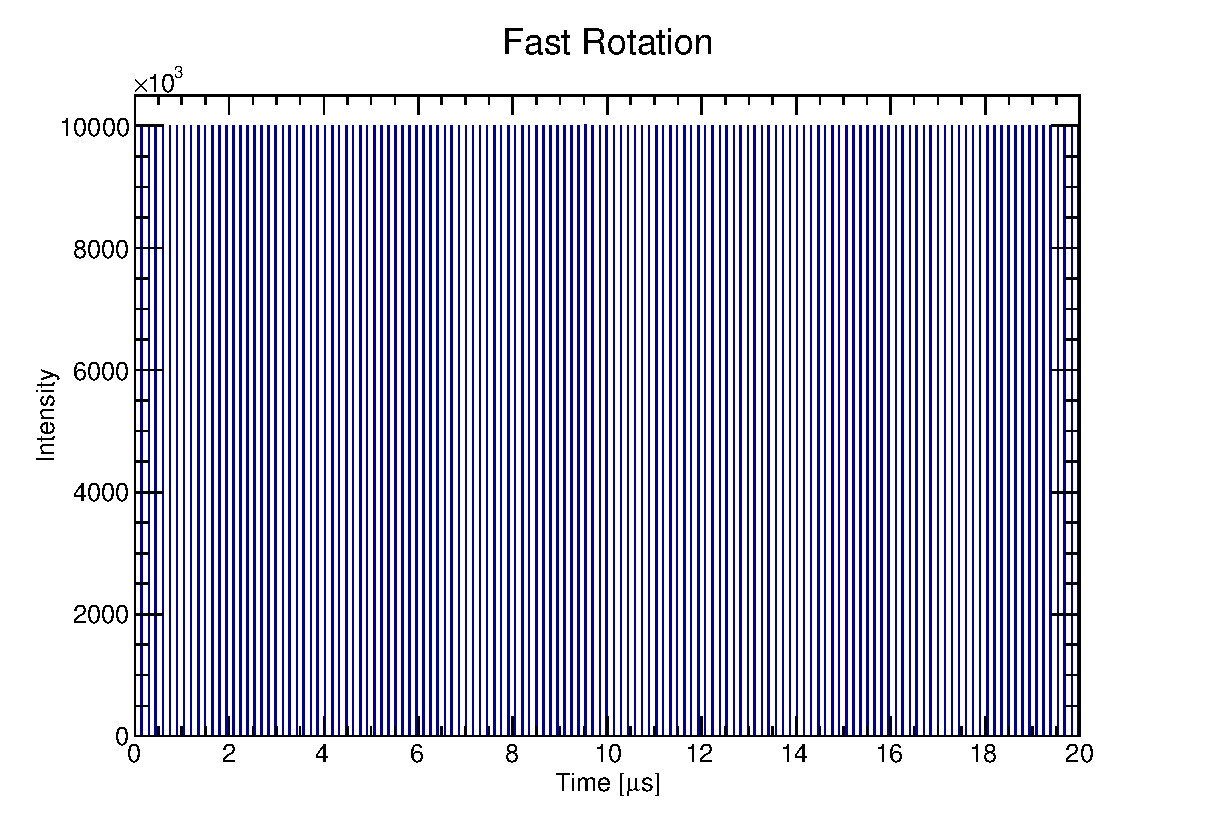
\includegraphics[width=0.45\textwidth]{fig/FRS_noSpread_0-20_us.eps}}
\subfigure[]{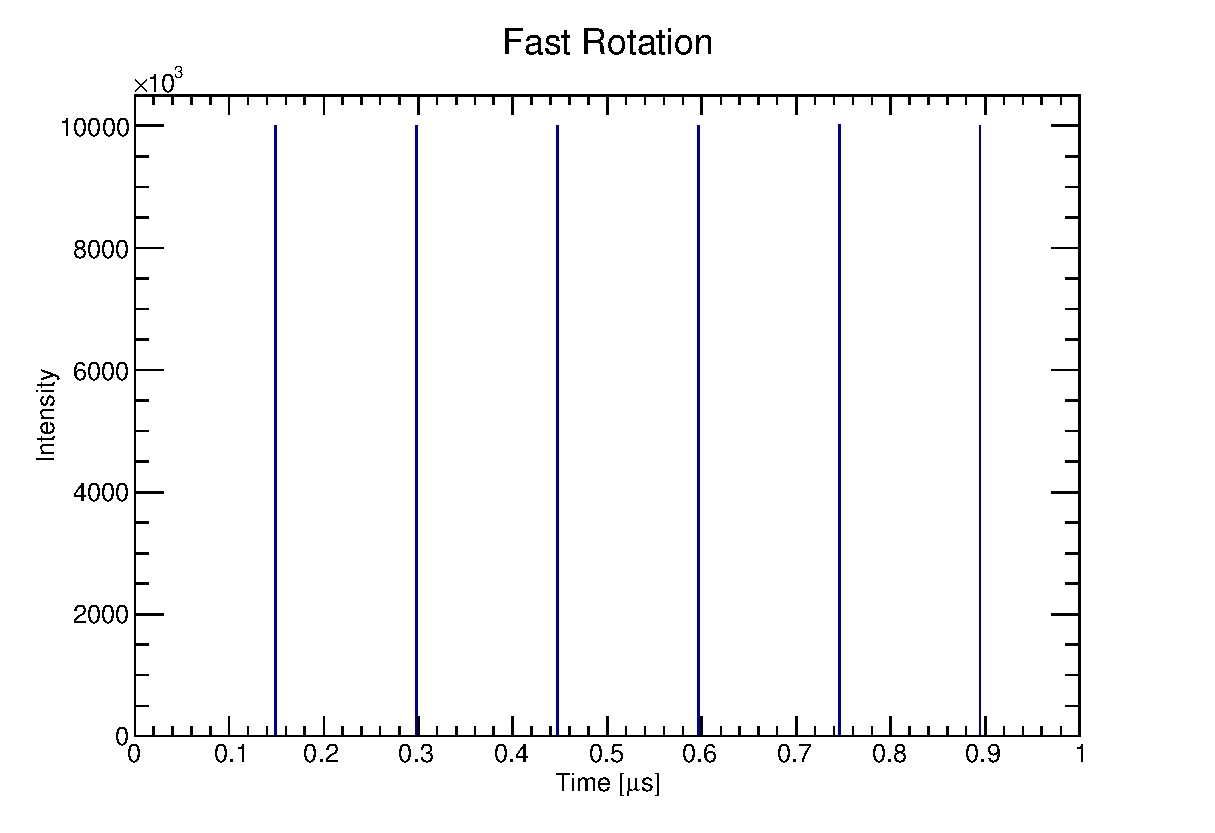
\includegraphics[width=0.45\textwidth]{fig/FRS_noSpread_0-1_us.eps}}
\caption{Fast rotation signal as a function of time for a muon beam with zero emittance, zero momentum spread and zero bunch length for two time windows: (a) 0-20 $\mu$s, (b) 0-1 $\mu$s.}
\label{fig:perfect_frs}
\end{figure}
 
A particle with momentum offset $\Delta$ will have revolution period $T(1+\Delta)$, so that 
\begin{equation}
I(t,\Delta)=\delta\left(t-\left(n+\frac{\theta}{2\pi}\right)T\left(1+\Delta\right)\right). 
\end{equation}
The fast rotation signal at the point is then~\footnote{the notation $(n+\frac{\theta}{2\pi})T$ will be noted thereafter $nT$ for improved text clarity} 

\begin{equation}
S(t)=\sum^{\infty}_{n=0}\int\rho(\Delta)\delta\left(t-nT\left(1+\Delta\right)\right)d\Delta 
\end{equation}
where $\rho(\Delta)$ is the distribution of momenta offsets. If the momentum distribution is a Gaussian with width $\Delta_0$, then 

\begin{eqnarray}
S(t) &=& \sum^{\infty}_{n=0}\int\frac{e^{-\Delta^2/(2\Delta^2_0)}}{\sqrt{2\pi}\Delta_0}
\delta\left(t-nT\left(1+\Delta\right)\right)d\Delta\\
&=&\sum^{\infty}_{n=0}\int\frac{e^{-\Delta^2/(2\Delta^2_0)}}{\sqrt{2\pi}\Delta_0}\frac{\delta\left(\Delta-\left(\frac{t}{nT}-1\right)\right)}{nT}d\Delta\\
&=&\sum^{\infty}_{n=0}\frac{e^{-(\frac{t}{nT}-1)^2/2\Delta^2_0}}{\sqrt{2\pi}\Delta_0nT}\label{eq:Espread_frs}
%&=&\sum^{\infty}_{n=0}\frac{e^{-(t-nT)^2/2\Delta^2_0(n+\theta/2\pi)^2T^2}}{\sqrt{2\pi}\Delta_0nT}\label{eq:Espread_frs}
\end{eqnarray}

Note that there is no muon decay in Eq.~(\ref{eq:Espread_frs}) or the accompanying plots.
Figure~\ref{fig:Espread_frs} shows the fast rotation signal for a beam with zero emittance, zero bunch length but with a 0.112\% momentum spread. 
One can see that the beam decoheres. The decoherence envelope is set by the momentum spread, the more spread the faster the decoherence.
The intensity asymptotically approaches that of the average stored current $<I> = eN\mu/T$.

\begin{figure}[bt]
\centering
\subfigure[]{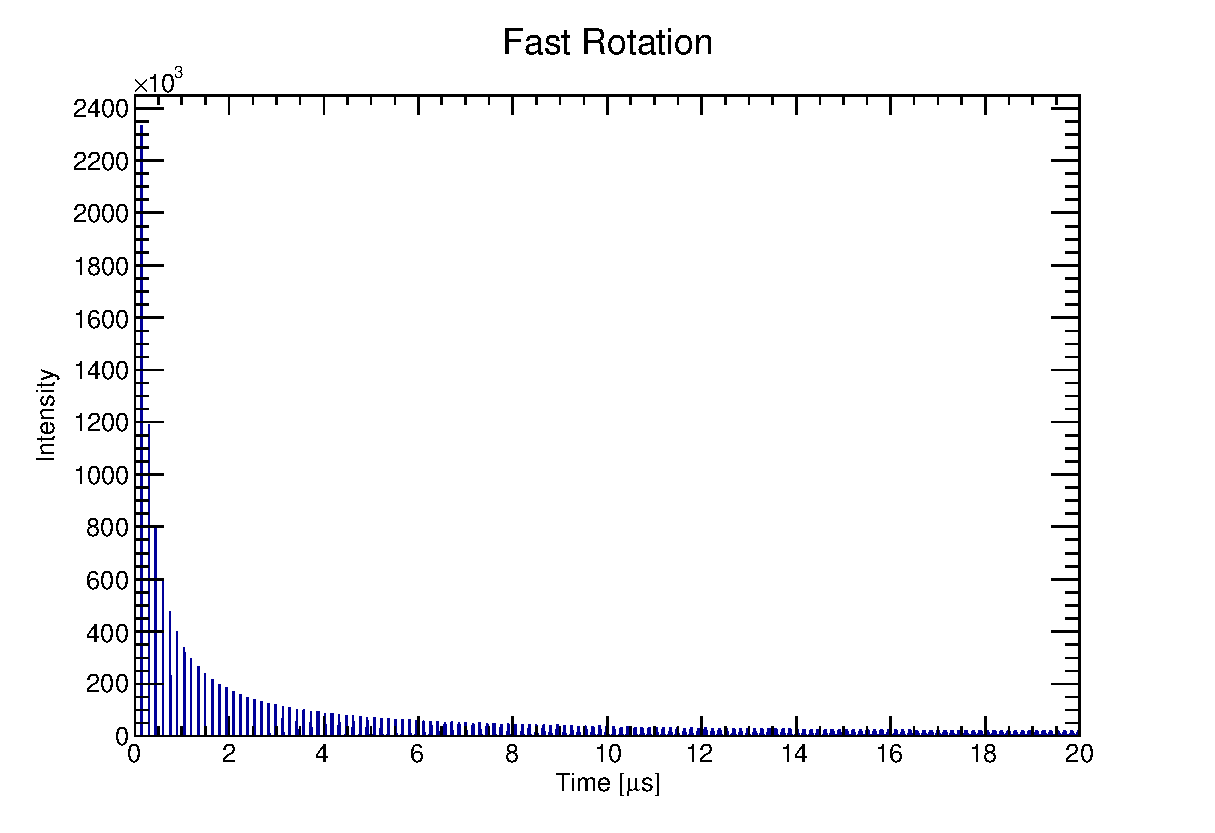
\includegraphics[width=0.6\textwidth]{fig/FRS_pSpread112_0-20us.eps}}\\
\subfigure[]{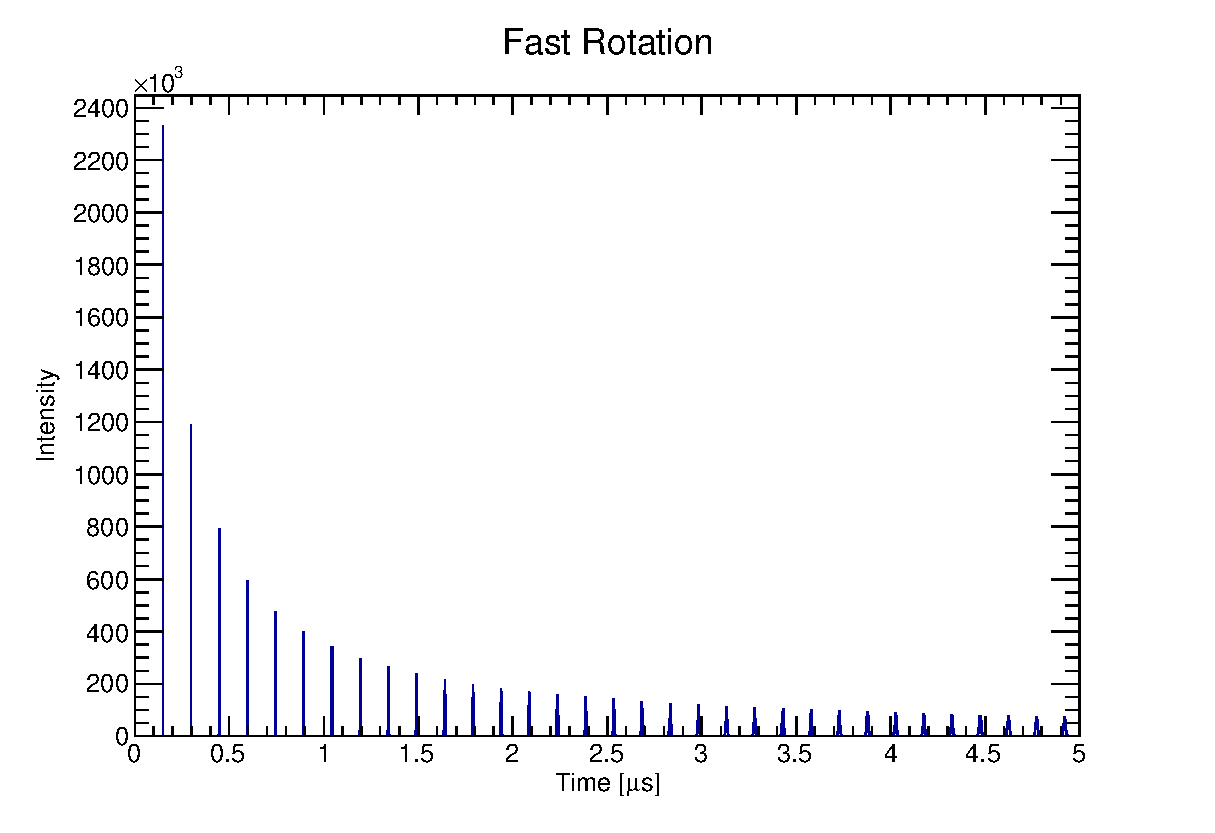
\includegraphics[width=0.45\textwidth]{fig/FRS_pSpread112_0-5us.eps}}
\subfigure[]{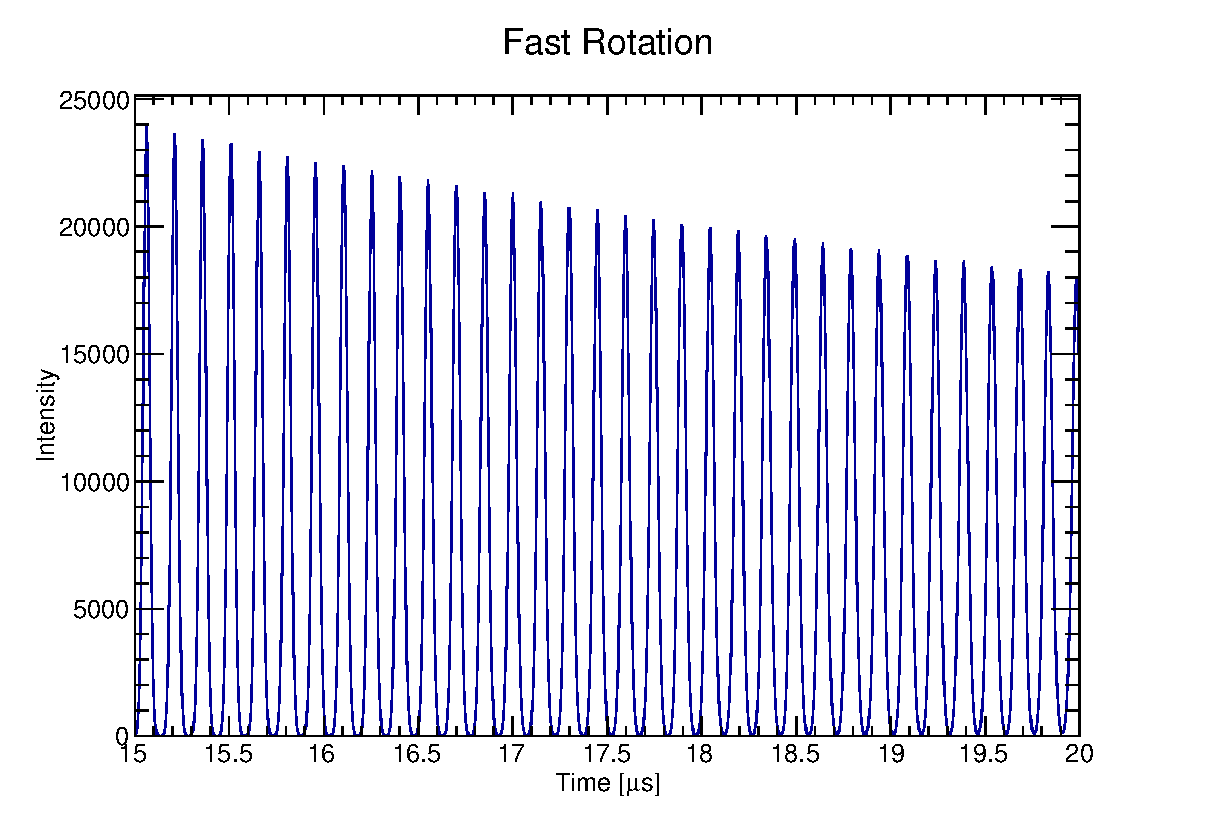
\includegraphics[width=0.45\textwidth]{fig/FRS_pSpread112_15-20us.eps}}
\caption{Fast rotation signal as a function of time for a muon beam with zero emittance, zero bunch length but width a 0.112\% momentum spread for three time windows: (a) 0-20 $\mu$s, (b) 0-5 $\mu$s, (c) 15-20 $\mu$s.}
\label{fig:Espread_frs}
\end{figure}

A realistic beam has, on top of the momentum spread, a non-zero bunch length. 
In this case Eq.~(\ref{eq:Espread_frs}) is re-expressed introducing a temporal offset $t^\prime$ as

\begin{eqnarray}
S(t,t^{\prime})&=& \sum_{n=0}^\infty\frac{e^{-(\frac{t-t^\prime}{nT}-1)^2/(2\Delta_0^2)}}{\sqrt{2\pi}\Delta_0 nT}.
\end{eqnarray}

Suppose the intial temporal (longitudinal) distribution of the muons is Gaussian 
$$\xi(t^\prime) = \frac{1}{\sqrt{2\pi}\sigma_t}e^{-{t^\prime}^2/(2\sigma_t^2)}$$.
Then
{\small
\begin{eqnarray*}
S(t)&=& \sum_{n=0}^\infty\int_{-\infty}^\infty dt^\prime \frac{e^{-(\frac{t-t^\prime}{nT}-1)^2/(2\Delta_0^2)}}{\sqrt{2\pi}\Delta_0 nT}\frac{1}{\sqrt{2\pi}\sigma_t}e^{-{t^\prime}^2/(2\sigma_t^2)}
\\
&=& \sum_{n=0}^\infty\frac{1}{2\pi\Delta_0nT\sigma_t}\int_{-\infty}^\infty dt^\prime e^{-(\frac{t-t^\prime}{nT}-1)^2/(2\Delta_0^2)}e^{-{t^\prime}^2/(2\sigma_t^2)}\\
%&=& \sum_{n=0}^\infty\frac{1}{2\pi\Delta_0(n+theta/2\pi)T\sigma_t}e^{-t^2/(2((n+theta/2\pi)T\Delta_0)^2)}
%\int_{-\infty}^\infty dt^\prime e^{-(\frac{{t^\prime}^2-2t t^\prime}{(nT)^2}+1 -\frac{2(t-t^\prime)}{nT})/(2\Delta_0^2)}e^{-{t^\prime}^2/(2\sigma_t^2)}\\
&=& \sum_{n=0}^\infty\frac{1}{2\pi\Delta_0nT\sigma_t}e^{-t^2/(2(nT\Delta_0)^2)}
\int_{-\infty}^\infty dt^\prime e^{-(\frac{{t^\prime}^2-2t t^\prime}{(nT)^2}+1 -\frac{2(t-t^\prime)}{nT})/(2\Delta_0^2)}e^{-{t^\prime}^2/(2\sigma_t^2)}\\
&=&\sum_{n=0}^\infty\frac{1}{2\pi\Delta_0nT\sigma_t}e^{-t^2/(2(nT\Delta_0)^2)}e^{\frac{t}{nT\Delta_0^2}}
\int_{-\infty}^\infty dt^\prime \exp(-{t^\prime}^2(\frac{1}{2(nT)^2\Delta_0^2}+\frac{1}{2\sigma_t^2})+t^\prime(\frac{t}{nT}-1)/(nT\Delta_0^2))e^{-1/(2\Delta_0^2)}\\
&=&\sum_{n=0}^\infty\frac{1}{2\pi\Delta_0nT\sigma_t}e^{-(\frac{t}{nT}-1)^2/2\Delta_0^2}
\int_{-\infty}^\infty dt^\prime \exp\left(-\alpha {t^\prime}^2+\beta t^\prime\right)\\
&=&\sum_{n=0}^\infty\frac{1}{2\pi\Delta_0nT\sigma_t}e^{-(\frac{t}{nT}-1)^2/(2\Delta_0^2)}
\sqrt{\frac{\pi}{\alpha}}e^{\beta^2/4\alpha},
\end{eqnarray*}
}
where $\alpha = \frac{1}{2(nT)^2\Delta_0^2}+\frac{1}{2\sigma_t^2}$ and $\beta= (\frac{t}{nT}-1)/(nT\Delta_0^2)$.
Finally
{\small
\begin{eqnarray}
S(t)&=&\sum_{n=0}^\infty\frac{1}{2\pi\Delta_0nT\sigma_t}e^{-(\frac{t}{nT}-1)^2/(2\Delta_0^2)}
\frac{\sqrt{2\pi}nT\Delta_0\sigma_t}{\sqrt{(nT)^2\Delta_0^2+\sigma_t^2}}
\exp(\frac{(\frac{t}{nT}-1)^2}{(nT\Delta_0^2)^2}\frac{(nT)^2\Delta_0^2\sigma_t^2}{2(nT)^2\Delta_0^2+2\sigma_t^2})\nonumber\\
&=& \frac{1}{\sqrt{2\pi}}\sum_{n=0}^\infty e^{-(\frac{t}{nT}-1)^2/(2\Delta_0^2)}
\frac{1}{\sqrt{((nT)^2\Delta_0^2+\sigma_t^2}}
\exp(\frac{(\frac{t}{nT}-1)^2}{\Delta_0^2}\frac{\sigma_t^2}{2(nT)^2\Delta_0^2+2\sigma_t^2})\nonumber\\
&=& \frac{1}{\sqrt{2\pi}}\sum_{n=0}^\infty
\frac{1}{\sqrt{((nT)^2\Delta_0^2+\sigma_t^2}}
\exp(\frac{-(\frac{t}{nT}-1)^2}{2\Delta_0^2}\left(1-\frac{\sigma_t^2}{(nT)^2\Delta_0^2+\sigma_t^2}\right).\label{eq:frs-sigt}
\end{eqnarray}
}


Figure~\ref{fig:E_T_spread_frs} shows the fast rotation signal for a beam with zero emittance, non-zero bunch length and non-zero momentum spread.
One can see that the beam decoheres faster having a longitudinal extension. It is expected since the longitudinal extension can be seen as 
created by a beam with an momentum spread having undergone an arbitrary number of revolution.

\begin{figure}[bt]
\centering
\subfigure[]{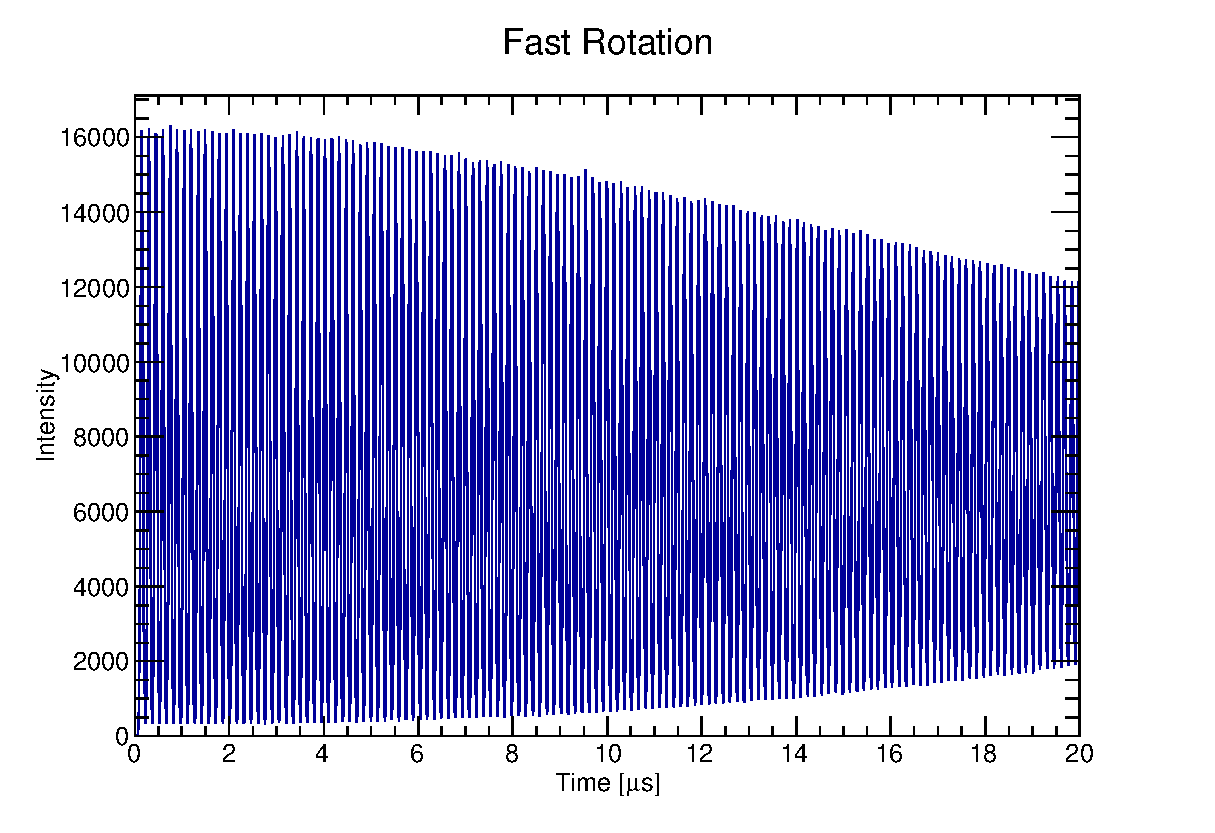
\includegraphics[width=0.6\textwidth]{fig/FRS_pSpread112_tSpread25ns_0-20us.eps}}\\
\subfigure[]{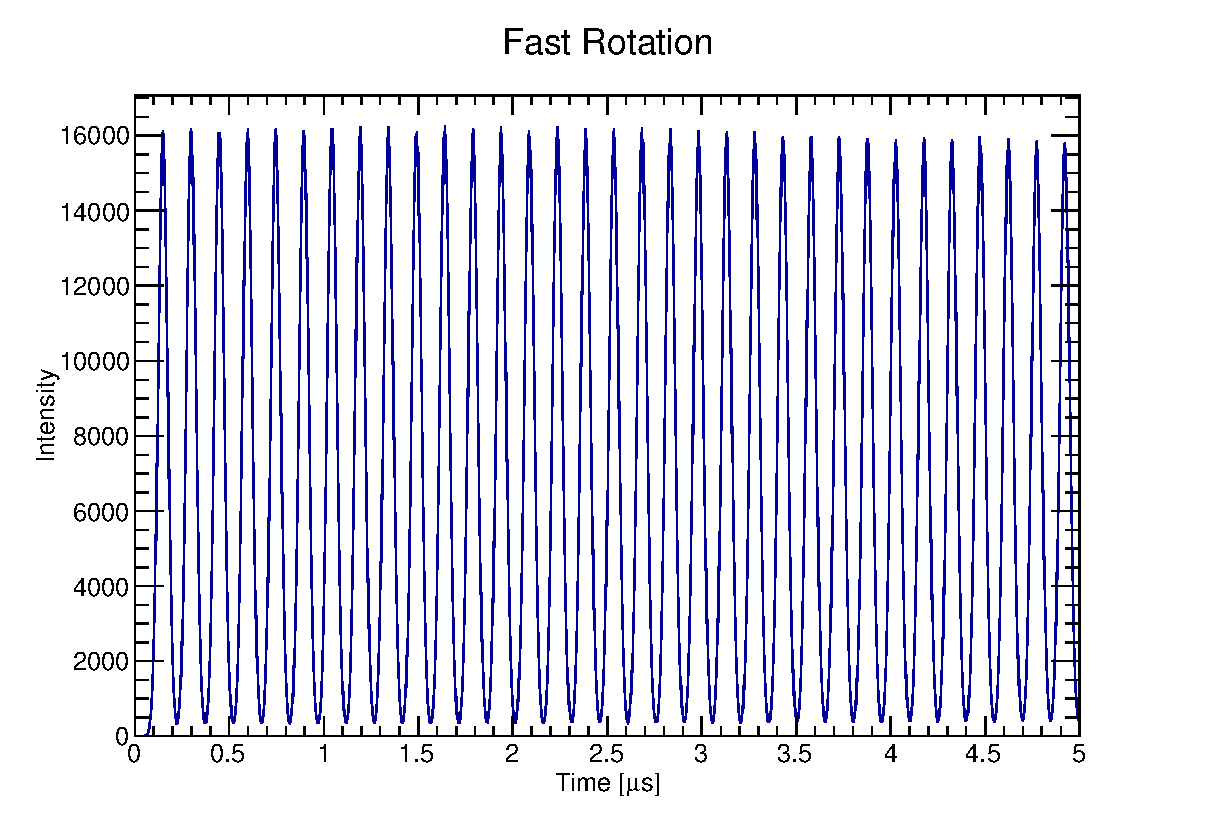
\includegraphics[width=0.45\textwidth]{fig/FRS_pSpread112_tSpread25ns_0-5us.eps}}
\subfigure[]{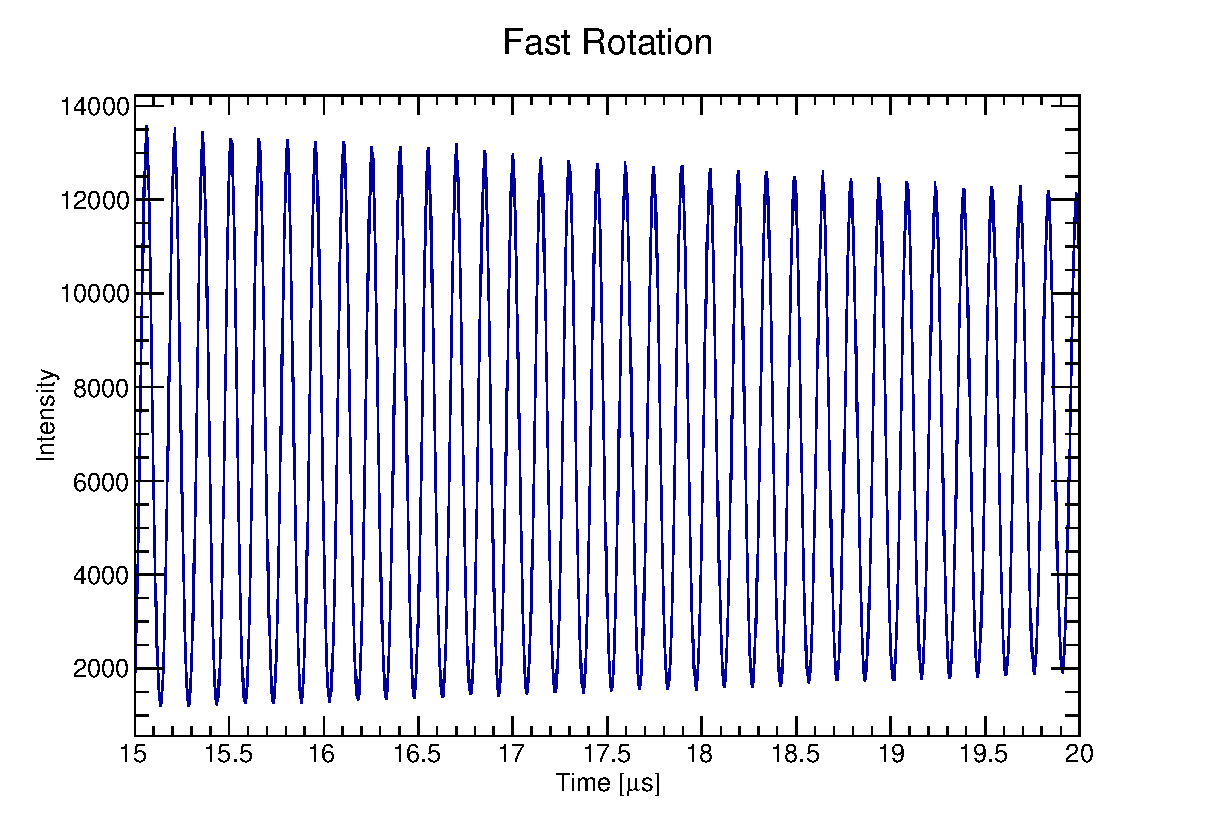
\includegraphics[width=0.45\textwidth]{fig/FRS_pSpread112_tSpread25ns_15-20us.eps}}
\caption{Fast rotation signal as a function of time for a muon beam with zero emittance, bunch length of 20 ns and momentum spread of 0.112\% for three time windows: (a) 0-20 $\mu$s, (b) 0-5 $\mu$s, (c) 15-20 $\mu$s.}
\label{fig:E_T_spread_frs}
\end{figure}


\newpage
\section{Theory of the Fourier Transform of the Fast Rotation Signal}

\subsection{Mathematical Preliminaries}

\begin{definition}[Fourier's transform and inverse transform]
Given a function $f$, its Fourier transform is \[\hat{f}(x)=\frac{1}{\sqrt{2\pi}}\int^{\infty}_{-\infty}f(t)e^{ixt}dt\] and its inverse Fourier transform is \[\tilde{f}(x)=\frac{1}{\sqrt{2\pi}}\int^{\infty}_{-\infty}f(t)e^{-ixt}dt\] If $f$ is absolutely integrable, then the Fourier transforms of $f$ always exist. It is easy to check that $f=\tilde{\hat{f}}=\hat{\tilde{f}}$.
\end{definition}

\begin{theorem}[Fourier's Integral]
For any piecewise continuous, piecewise differentiable, and absolutely integrable function $f$, the following equality holds: \[f(x)=\frac{1}{\pi}\int^{\infty}_0d\omega\int^{\infty}_{-\infty}f(t)\cos\omega(t-x)dt\]
\end{theorem}

If $f$ is even, then Fourier's integral simplifies to \[f(x)=\frac{2}{\pi}\int^{\infty}_0\cos\omega xd\omega\int^{\infty}_0f(t)\cos\omega tdt\]Suppose $f$ is a piecewise continuous, piecewise differentiable, and absolutely integrable function on $[0,\infty)$. If we extend $f$ to an even function defined on the whole real line, then the formula above is valid for the extension. In particular, it is also valid for $x\geq 0$.

\begin{theorem}[Convolution Theorem]
The convolution of two functions $f$ and $g$ is defined to be \[(f\ast g)(t)=\frac{1}{\sqrt{2\pi}}\int^{\infty}_{-\infty}f(\tau)g(t-\tau)d\tau\] The convolution theorem states that \[\widehat{f\ast g}=\hat{f}\hat{g} \text{ and } \widetilde{f\ast g}=\tilde{f}\tilde{g}\] 
\end{theorem}

%Suppose the supports of $f$ and $g$ are $(t_1,t_2)$ and $(t_3,t_4)$, respectively. Then \[(f\ast g)(t)=\int^{\infty}_{-\infty}f(\tau)g(t-\tau)d\tau=\int^{t_2}_{t_1}f(\tau)g(t-\tau)d\tau\] As $\tau$ increases from $t_1$ to $t_2$, the argument of $g(t-\tau)$ decreases from $t-t_1$ to $t-t_2$. Therefore the integrand vanishes if $t$ is such that $t-t_1<t_3$ or $t-t_2>t_4$. Hence the support of $(f\ast g)(t)$ is $(t_1+t_3,t_2+t_4)$.%

\subsection{The case of initially zero bunch length}

In this case we have that $\xi(t')=\delta(t')$, so the fast rotation signal becomes \[S(t)=\sum^{\infty}_{n=0}\frac{\rho\left(\frac{t}{(n+\theta/2\pi)T}-1\right)}{(n+\theta/2\pi)T}\]
Assuming the bunch evolves such that in the first turn the beam spreads negligibly, the center of mass of the bunch reaches the fiber harp at position $\theta$ at some time $t_0$. This $t_0$ is the time when muons at the magic frequency first reach the detector. Furthermore, we have that $\theta/2\pi=t_0/T$, so we may write 

\[
S(t)=\sum^{\infty}_{n=0}\frac{\rho\left(\frac{t}{nT+t_0}-1\right)}{nT+t_0}
\]
We next assume that $\mathcal{S}(t)\equiv S(t+t_0)$ is sufficiently well behaved so as to be absolutely integrable on $[0,\infty)$, as well as piecewise continuous and piecewise differentiable. Note that this means that $\rho(\Delta)$ must satisfy these conditions also. Extend $\mathcal{S}$ to the entire real line as an even function. By Theorem 1, we may express $\mathcal{S}$ as \[\mathcal{S}(t)=\frac{2}{\pi}\int^{\infty}_0\cos\omega td\omega\int^{\infty}_0\mathcal{S}(t')\cos\omega t'dt'\] We then recover $S(t)$:\[S(t+t_0)=\frac{2}{\pi}\int^{\infty}_0\cos\omega td\omega\int^{\infty}_0S(t'+t_0)\cos\omega t'dt'=\]\[\frac{2}{\pi}\int^{\infty}_0\cos\omega td\omega\int^{\infty}_{t_0}S(t')\cos\omega(t'-t_0)dt'\Rightarrow\]

\[
S(t)=\frac{2}{\pi}\int^{\infty}_0\cos\omega(t-t_0)d\omega\int^{\infty}_{t_0}S(t')\cos\omega(t'-t_0)dt'
\] 
But we also know from Definition 1 that \[\mathcal{S}(t)=\tilde{\hat{\mathcal{S}}}(t)=\frac{1}{2\pi}\int^{\infty}_{-\infty}e^{-i\omega t}d\omega\int^{\infty}_{-\infty}\mathcal{S}(t')e^{i\omega t'}dt'=\]\[\frac{1}{2\pi}\int^{\infty}_{-\infty}e^{-i\omega t}d\omega\int^{\infty}_{-\infty}\mathcal{S}(t')(\cos\omega t'+i\sin\omega t')dt'=\frac{1}{2\pi}\int^{\infty}_{-\infty}e^{-i\omega t}d\omega\int^{\infty}_{-\infty}\mathcal{S}(t')\cos\omega t'dt'\] where we used the fact that $\mathcal{S}$ is an even function, and the integral of the product of an even and odd function vanishes. From the preceding expression we now see that $\hat{\mathcal{S}}$ is an even function. So we write \[\frac{1}{2\pi}\int^{\infty}_{-\infty}\hat{\mathcal{S}}(\omega)\cos\omega td\omega=\frac{1}{\pi}\int^{\infty}_0\hat{\mathcal{S}}(\omega)\cos\omega td\omega=\frac{2}{\pi}\int^{\infty}_0\cos\omega td\omega\int^{\infty}_0\mathcal{S}(t')\cos\omega t'dt'\] Thus 

\begin{equation}
\hat{S}(\omega)=\sqrt{\frac{2}{\pi}}\int^{\infty}_{t_0}S(t)\cos\omega(t-t_0)dt
\label{eq:nospreadFT}
\end{equation} 
is the Fourier transform of $S$. So if we're given $\hat{S}(\omega)$, we may express $S$ as 

\begin{equation}
S(t)=\sqrt{\frac{2}{\pi}}\int^{\infty}_0\hat{S}(\omega)\cos\omega(t-t_0)d\omega=\frac{1}{\sqrt{2\pi}}\int^{\infty}_{-\infty}\hat{S}(\omega)\cos\omega(t-t_0)d\omega
\label{eq:nospreadIFT}
\end{equation}

\subsection{Bunch Length Distribution $\xi(t')$}
We call the fast rotation signal with no inital bunch length $S_0(t)$. Given an initial longitudinal distribution $\xi(t')$, the fast rotation signal is described by \[S(t)=\int\xi(t')S_0(t-t')dt'=\sqrt{2\pi}(\xi\ast S_0)(t)\] In the ideal case we would directly apply the convolution theorem to find that 

\begin{equation}
\hat{S}(\omega)=\sqrt{2\pi}\hat{\xi}(\omega)\hat{S}_0(\omega)
\label{eq:ConvoSpectrum}
\end{equation} However, we won't have $S_0(t)$ to work with directly, nor $\xi(t)$. We need to use $S(t)$ to get $\hat{S}(\omega)$. 

We express $S_0(t-t')$ through Fourier's integral: \[S_0(t-t')=\frac{2}{\pi}\int^{\infty}_0\cos\omega(t-t_0-t')d\omega\int^{\infty}_{t_0}S_0(\bar{t})\cos\omega(\bar{t}-t_0)d\bar{t}=\]\[\sqrt{\frac{2}{\pi}}\int^{\infty}_0\hat{S}_0(\omega)\cos\omega(t-t_0-t')d\omega\] Substituting this expression into the convolution integral, we get \[S(t)=(\xi\ast S_0)(t)=\int^{\infty}_{-\infty}\xi(t)S_0(t-t')dt'=\sqrt{\frac{2}{\pi}}\int^{\infty}_0\hat{S}_0(\omega)d\omega\int^{\infty}_{-\infty}\xi(t')\cos\omega(t-t_0-t')dt'=\]\[\sqrt{\frac{2}{\pi}}\int^{\infty}_0\hat{S}_0(\omega)\langle\cos\omega(t-t_0-t')\rangle d\omega=\]\[\sqrt{\frac{2}{\pi}}\int^{\infty}_0\hat{S}_0(\omega)\langle\cos\omega(t-t_0)\cos\omega t'+\sin\omega(t-t_0)\sin\omega t'\rangle d\omega=\]\[\sqrt{\frac{2}{\pi}}\left(\int^{\infty}_0\hat{S}_0(\omega)\langle\cos\omega t'\rangle\cos\omega(t-t_0)d\omega+\int^{\infty}_0\hat{S}_0(\omega)\langle\sin\omega t'\rangle\sin\omega(t-t_0)d\omega\right)\] where $\langle\text{ }\rangle$ denotes averaging with respect to $\xi(t)$. 

If $\xi(t')$ is even, $\langle\sin\omega t'\rangle=0$. We are then left with 

\begin{equation}
S(t)=\sqrt{\frac{2}{\pi}}\int^{\infty}_0\hat{S}_0(\omega)\langle\cos\omega t'\rangle\cos\omega(t-t_0)d\omega
\label{eq:EvenBunchFT}
\end{equation} suggesting that $\hat{S}(\omega)=\hat{S}_0(\omega)\langle\cos\omega t'\rangle$. We can see that this is true by looking back at$~\eqref{eq:ConvoSpectrum}$: \[\hat{\xi}(\omega)=\frac{1}{\sqrt{2\pi}}\int^{\infty}_{-\infty}\xi(t')e^{i\omega t'}dt'=\frac{1}{\sqrt{2\pi}}\int^{\infty}_{-\infty}\xi(t')\cos\omega t'dt'=\frac{\langle\cos\omega t'\rangle}{\sqrt{2\pi}}\] and therefore $\hat{S}(\omega)=\sqrt{2\pi}\hat{\xi}(\omega)\hat{S}_0(\omega)=\hat{S}_0(\omega)\langle\cos\omega t'\rangle$. Thus $~\eqref{eq:EvenBunchFT}$ is the inverse Fourier transform, implying that \[\hat{S}(\omega)=\sqrt{\frac{2}{\pi}}\int^{\infty}_{t_0}S(t)\cos\omega(t-t_0)dt\] 

If $\xi(t')$ is not symmetric, then we are faced with the problem that $\hat{S}(\omega)$ features an imaginary component.

\subsection{Corrections to the Fourier Transform}

If the detector detects the muons at a time $t_s>t_0$, then the resulting Fourier transform of the observed fast rotation signal has a missing component 
\begin{equation}
\Delta(\omega)=\sqrt{\frac{2}{\pi}}\int^{t_s}_{t_0}S(t)\cos\omega(t-t_0)dt
\label{eq:Delta}
\end{equation} while the immediately observed frequency spectrum is 

\begin{equation}
\hat{S}(\omega)=\sqrt{\frac{2}{\pi}}\int^{\infty}_{t_s}S(t)\cos\omega(t-t_0)dt
\label{eq:firstapprox}
\end{equation}
However, we do not observe $S(t)$ on $(t_0,t_s)$, so we need to find a way to correct the frequency spectrum. 

In order to do this, we first note that the Fourier transform has associated with it an uncertainty principle, namely that $\Delta f\Delta t\sim1$. If $t_s$ isn't too great, we can then expect that the spread of $\Delta(\omega)$ about the magic frequency will be large while the spread of $\hat{S}(\omega)$ will change negligibly. So we may express $S(t)$ using the observed $\hat{S}(\omega)$ through formula$~\eqref{eq:nospreadIFT}$. Thus we have that \[\Delta(\omega)=\frac{2}{\pi}\int^{t_s}_{t_0}\int^{\infty}_0\hat{S}(\omega')\cos\omega'(t-t_0)\cos\omega(t-t_0)d\omega' dt\] Integrating with respect to $t$ first, we get \[\Delta(\omega)=\frac{1}{\pi}\int^{\infty}_0\hat{S}(\omega)\left(\frac{\sin(\omega-\omega')(t_s-t_0)}{\omega-\omega'}+\frac{\sin(\omega+\omega')(t_s-t_0)}{\omega+\omega'}\right)d\omega'\] We may neglect the second term in the parentheses, as we are interested in frequencies $\omega$ such that $|\omega-\omega'|<<\omega+\omega'$, so 

\begin{equation}
\Delta(\omega)=\frac{1}{\pi}\int^{\infty}_0\hat{S}(\omega)\frac{\sin(\omega-\omega')(t_s-t_0)}{\omega-\omega'}d\omega'
\label{eq:approxDelta}
\end{equation}

\subsection{Physical Interpretation of the Fourier Transform of the Fast Rotation Signal}

Assuming that the energy offset distribution $\rho(\Delta)$ is centered with a maximum at $\Delta=0$, the harmonics of the Fourier transform of the fast rotation signal will be featured at integer multiples of the magic frequency; this is evident from the construction of the general fast rotation signal. The signal is due to the orbits of muons at various revolution frequencies, so $\hat{S}(\omega)$ describes the distribution of revolution frequencies among the muons. However, the muons are restricted to the vacuum chamber, making frequencies corresponding to muons outside the chamber nonphysical. Hence the first harmonic corresponds to the physical revolution frequency distribution of the muons.

\section{Analysis for a Gaussian Energy Offset Distribution and Initially Zero Bunch Length}

If the energy offset distribution is a Gaussian with width $\Delta_0$, then \[S(t)=\sum^{\infty}_{n=0}\frac{e^{-(t-(nT+t_0))^2/2\Delta^2_0(nT+t_0)^2}}{\sqrt{2\pi}\Delta_0(nT+t_0)}\] Suppose the center of mass of the muon beam first passes the detector at time $t_0$, and the detector starts detecting at some time $t_s>t_0$. Then the Fourier transform of the fast rotation signal is

\begin{gather}
\hat{S}(\omega)=\sqrt{\frac{2}{\pi}}\int^{\infty}_{t_s}S(t)\cos\omega(t-t_0) dt \nonumber \\
=\sqrt{\frac{2}{\pi}}\sum^{\infty}_{n=0}\int^{\infty}_{t_s}\frac{e^{-(t-(nT+t_0))^2/2\Delta^2_0(nT+t_0)^2}}{\sqrt{2\pi}\Delta_0(nT+t_0)}\cos\omega(t-t_0)dt \nonumber \\ 
=\sqrt{\frac{2}{\pi}}\sum^{\infty}_{n=0}\frac{e^{-1/2\Delta^2_0}}{2\sqrt{2\pi}\Delta_0(nT+t_0)}\int^{\infty}_{t_s}e^{-t^2/2\Delta^2_0(nT+t_0)^2}e^{t/(nT+t_0)\Delta^2_0}e^{\pm i\omega t}e^{\mp i\omega t_0}dt.
\end{gather}

From Gradshteyn and Rizhik, we know that 
\begin{equation}
\int^{\infty}_u\exp\left(-\frac{x^2}{4\beta}-\gamma x\right)dx=\sqrt{\pi\beta}e^{\beta\gamma^2}\left(1-\frac{\sqrt{\pi}}{2}\text{Erf}\left(\gamma\sqrt{\beta}+\frac{u}{2\sqrt{\beta}}\right)\right)
\label{eq:GradRyzhik}
\end{equation}
for $\text{Re}(\beta)>0$ and $u\geq0$. Thus the result of using this integral in computing the Fourier transform is $\hat{S}(\omega)=$ 

\begin{gather}
\sqrt{\frac{2}{\pi}}\sum^{\infty}_{n=0}\frac{e^{-\omega^2(nT+t_0)^2\Delta^2_0/2}e^{i\omega nT}}{4}\left(1-\frac{\sqrt{\pi}}{2}\text{Erf}\left[\frac{-1}{\Delta_0\sqrt{2}}-\frac{i\omega (nT+t_0)\Delta_0}{\sqrt{2}}+\frac{t_s}{\Delta_0(nT+t_0)\sqrt{2}}\right]\right)+ \nonumber \\
\sqrt{\frac{2}{\pi}}\sum^{\infty}_{n=0}\frac{e^{-\omega^2(nT+t_0)^2\Delta^2_0/2}e^{-i\omega nT}}{4}\left(1-\frac{\sqrt{\pi}}{2}\text{Erf}\left[\frac{-1}{\Delta_0\sqrt{2}}+\frac{i\omega (nT+t_0)\Delta_0}{\sqrt{2}}+\frac{t_s}{\Delta_0(nT+t_0)\sqrt{2}}\right]\right)
\end{gather}

\subsection{Corrections to the Fourier transform} The detector in the section above started to detect the muon beam at a time $t_s>t_0$. This results in some lost frequency content in the Fourier transform above, creating distortions of the frequency spectrum. The missing part of the frequency spectrum is described by formula$~\eqref{eq:Delta}$. Let's take a closer look at $\Delta$. \[\Delta(\omega)=\sqrt{\frac{2}{\pi}}\int^{t_s}_{t_0}S(t)\cos\omega(t-t_0)dt\]\[=\sqrt{\frac{2}{\pi}}\int^{\infty}_{t_0}S(t)\cos\omega(t-t_0)dt-\sqrt{\frac{2}{\pi}}\int^{\infty}_{t_s}S(t)\cos\omega(t-t_0)dt\] Using$~\eqref{eq:GradRyzhik}$, we have 

\begin{gather}
\sqrt{\frac{2}{\pi}}\sum^{\infty}_{n=0}\frac{e^{-\omega^2(nT+t_0)^2\Delta^2_0/2}e^{i\omega nT}}{4}\left(1-\frac{\sqrt{\pi}}{2}\text{Erf}\left[\frac{-1}{\Delta_0\sqrt{2}}-\frac{i\omega (nT+t_0)\Delta_0}{\sqrt{2}}+\frac{t_0}{\Delta_0(nT+t_0)\sqrt{2}}\right]\right)+ \nonumber \\
\sqrt{\frac{2}{\pi}}\sum^{\infty}_{n=0}\frac{e^{-\omega^2(nT+t_0)^2\Delta^2_0/2}e^{-i\omega nT}}{4}\left(1-\frac{\sqrt{\pi}}{2}\text{Erf}\left[\frac{-1}{\Delta_0\sqrt{2}}+\frac{i\omega (nT+t_0)\Delta_0}{\sqrt{2}}+\frac{t_0}{\Delta_0(nT+t_0)\sqrt{2}}\right]\right) \nonumber \\
-\sqrt{\frac{2}{\pi}}\sum^{\infty}_{n=0}\frac{e^{-\omega^2(nT+t_0)^2\Delta^2_0/2}e^{i\omega nT}}{4}\left(1-\frac{\sqrt{\pi}}{2}\text{Erf}\left[\frac{-1}{\Delta_0\sqrt{2}}-\frac{i\omega (nT+t_0)\Delta_0}{\sqrt{2}}+\frac{t_s}{\Delta_0(nT+t_0)\sqrt{2}}\right]\right)+ \nonumber \\
-\sqrt{\frac{2}{\pi}}\sum^{\infty}_{n=0}\frac{e^{-\omega^2(nT+t_0)^2\Delta^2_0/2}e^{-i\omega nT}}{4}\left(1-\frac{\sqrt{\pi}}{2}\text{Erf}\left[\frac{-1}{\Delta_0\sqrt{2}}+\frac{i\omega (nT+t_0)\Delta_0}{\sqrt{2}}+\frac{t_s}{\Delta_0(nT+t_0)\sqrt{2}}\right]\right)
\end{gather}

\begin{figure}[ht]
\centering
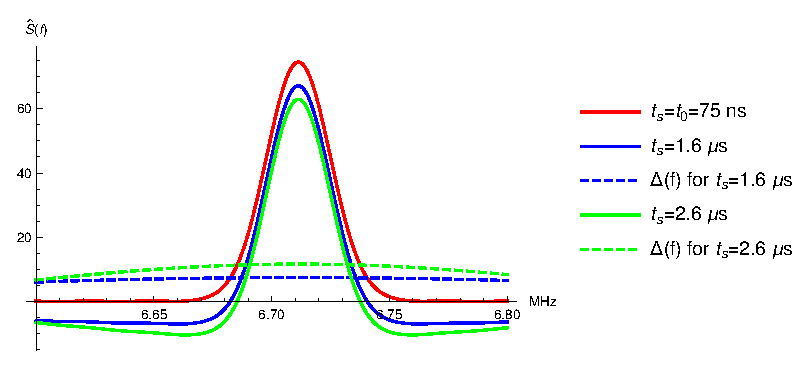
\includegraphics[scale=0.6]{fig/FT_no_tspread.eps}
\caption{Frequency spectra for the case of a Gaussian energy offset distribution and no initial bunch length. Spectra for different $t_s$ are displayed, as well the corresponding $\Delta(f)$ functions}
\end{figure}

Figure~\ref{fig:FT_no_tspread} shows how the Fourier transform and the corresponding corrections are altered by increasing $t_s$.

\section{Analysis for a Gaussian Energy Offset Distribution and Gaussian Longitudinal Distribution}

The fast rotation signal in this case is of the same form as in the case of no longitudinal distribution: \[S(t)=\sum^{\infty}_{n=0}\frac{e^{-(t-(nT+t_0))^2/2\Delta'^2_0(nT+t_0)^2}}{\sqrt{2\pi}\Delta'_0(nT+t_0)}\] Thus $\hat{S}(\omega)=$ 

\begin{gather}
\sqrt{\frac{2}{\pi}}\sum^{\infty}_{n=0}\frac{e^{-\omega^2(nT+t_0)^2\Delta'^2_0/2}e^{i\omega nT}}{4}\left(1-\frac{\sqrt{\pi}}{2}\text{Erf}\left[\frac{-1}{\Delta'_0\sqrt{2}}-\frac{i\omega (nT+t_0)\Delta'_0}{\sqrt{2}}+\frac{t_s}{\Delta'_0(nT+t_0)\sqrt{2}}\right]\right)+ \nonumber \\
\sqrt{\frac{2}{\pi}}\sum^{\infty}_{n=0}\frac{e^{-\omega^2(nT+t_0)^2\Delta'^2_0/2}e^{-i\omega nT}}{4}\left(1-\frac{\sqrt{\pi}}{2}\text{Erf}\left[\frac{-1}{\Delta'_0\sqrt{2}}+\frac{i\omega (nT+t_0)\Delta'_0}{\sqrt{2}}+\frac{t_s}{\Delta'_0(nT+t_0)\sqrt{2}}\right]\right)
\end{gather}
and $\Delta(\omega)=$
\begin{gather}
\sqrt{\frac{2}{\pi}}\sum^{\infty}_{n=0}\frac{e^{-\omega^2(nT+t_0)^2\Delta'^2_0/2}e^{i\omega nT}}{4}\left(1-\frac{\sqrt{\pi}}{2}\text{Erf}\left[\frac{-1}{\Delta'_0\sqrt{2}}-\frac{i\omega (nT+t_0)\Delta'_0}{\sqrt{2}}+\frac{t_0}{\Delta'_0(nT+t_0)\sqrt{2}}\right]\right)+ \nonumber \\
\sqrt{\frac{2}{\pi}}\sum^{\infty}_{n=0}\frac{e^{-\omega^2(nT+t_0)^2\Delta'^2_0/2}e^{-i\omega nT}}{4}\left(1-\frac{\sqrt{\pi}}{2}\text{Erf}\left[\frac{-1}{\Delta_0\sqrt{2}}+\frac{i\omega (nT+t_0)\Delta'_0}{\sqrt{2}}+\frac{t_0}{\Delta'_0(nT+t_0)\sqrt{2}}\right]\right) \nonumber \\
-\sqrt{\frac{2}{\pi}}\sum^{\infty}_{n=0}\frac{e^{-\omega^2(nT+t_0)^2\Delta'^2_0/2}e^{i\omega nT}}{4}\left(1-\frac{\sqrt{\pi}}{2}\text{Erf}\left[\frac{-1}{\Delta_0\sqrt{2}}-\frac{i\omega (nT+t_0)\Delta'_0}{\sqrt{2}}+\frac{t_s}{\Delta'_0(nT+t_0)\sqrt{2}}\right]\right)+ \nonumber \\
-\sqrt{\frac{2}{\pi}}\sum^{\infty}_{n=0}\frac{e^{-\omega^2(nT+t_0)^2\Delta'^2_0/2}e^{-i\omega nT}}{4}\left(1-\frac{\sqrt{\pi}}{2}\text{Erf}\left[\frac{-1}{\Delta_0\sqrt{2}}+\frac{i\omega (nT+t_0)\Delta'_0}{\sqrt{2}}+\frac{t_s}{\Delta'_0(nT+t_0)\sqrt{2}}\right]\right)
\end{gather}

\begin{figure}[ht]
\centering
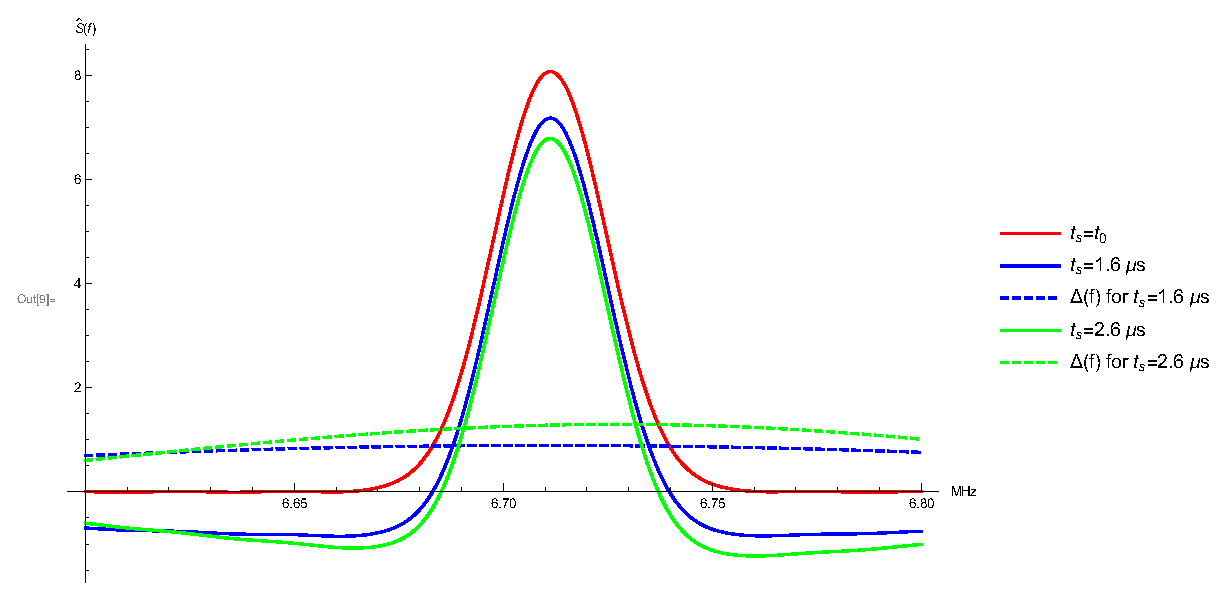
\includegraphics[scale=1.0]{fig/FT_tspread.eps}
\caption{Frequency spectra for the case of a Gaussian energy offset distribution and Gaussian bunch length distribution. Spectra for different $t_s$ are displayed, as well the corresponding $\Delta(f)$ functions}
\label{fig:FT_tspread}
\end{figure}

Figure~\ref{fig:FT_tspread} shows how the Fourier transform and the corresponding corrections are altered by increasing $t_s$.


\begin{thebibliography}{}

\bibitem{orlov}
Y. Orlov et al., NIM A 482 (2002) 767-755.

\end{thebibliography}


\end{document}
